% 图 26.3 —— 由 `checks/emit_hand.py` 自动拼出（probe 精测 + prims2 图元分解）
%%
% ⚠ 这是**稿子不是成品**：跑 `checks/checkhand.py 26.3` 看指标 + 看叠合图。
%%
%% ⚠ 待核：
%   · 本图 probe 报出阴影族 5 个 —— **本脚本不生成阴影**（要照原书手写）；prims2 的 strokes 里可能含阴影线，核对时留意别画重
%   · 可疑字形 1 项（空心圈 ⊙ 常被认成字母 o）—— 见文件末
%%
\documentclass[12pt]{standalone}
\usepackage{fontspec}
\setsansfont{Arial}
\newfontfamily\mfallback{DejaVu Sans}
\usepackage{tikz}
\begin{document}
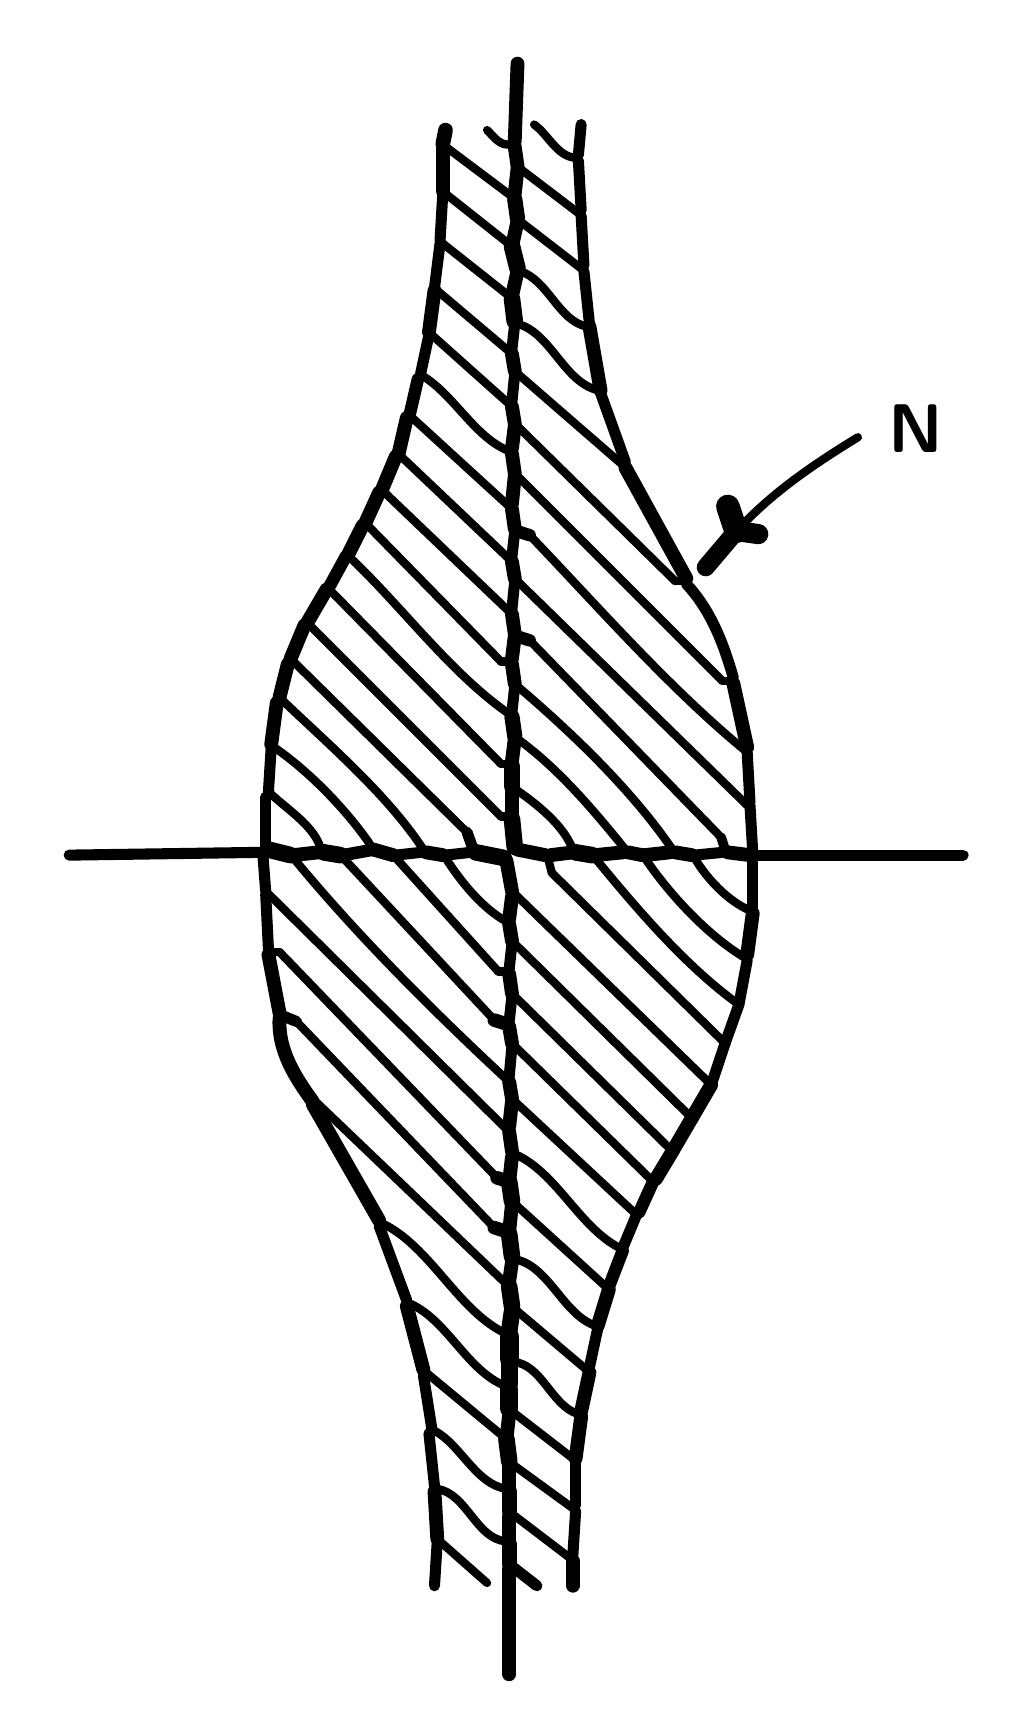
\begin{tikzpicture}[x=1pt, y=-1pt, line width=4.0pt, line cap=round, line join=round]

  %% ════ 直线段（prims2 的 strokes）════
  \draw[line width=4.0pt] (175.0,135.0) -- (176.0,125.0);
  \draw[line width=3.0pt] (148.0,95.0) -- (174.0,117.0);
  \draw[line width=7.0pt] (174.0,481.0) -- (174.0,473.0);
  \draw[line width=5.0pt] (203.0,108.0) -- (207.0,131.0);
  \draw[line width=5.0pt] (175.0,97.0) -- (177.0,88.0);
  \draw[line width=5.0pt] (174.0,538.0) -- (174.0,546.0);
  \draw[line width=4.0pt] (200.0,35.0) -- (199.0,46.0);
  \draw[line width=4.0pt] (203.0,484.0) -- (206.0,470.0);
  \draw[line width=3.0pt] (104.0,388.0) -- (173.0,454.0);
  \draw[line width=5.0pt] (175.0,154.0) -- (176.0,161.0);
  \draw[line width=6.0pt] (175.0,444.0) -- (174.0,436.0);
  \draw[line width=5.0pt] (175.0,193.0) -- (176.0,199.0);
  \draw[line width=5.0pt] (150.0,44.0) -- (150.0,59.0);
  \draw[line width=5.0pt] (176.0,60.0) -- (177.0,51.0);
  \draw[line width=5.0pt] (175.0,367.0) -- (174.0,361.0);
  \draw[line width=4.0pt] (175.0,116.0) -- (176.0,107.0);
  \draw[line width=3.0pt] (174.0,211.0) -- (129.0,168.0);
  \draw[line width=3.0pt] (260.0,281.0) -- (177.0,200.0);
  \draw[line width=4.5pt] (125.0,297.0) -- (114.0,299.0);
  \draw[line width=5.0pt] (125.0,297.0) -- (132.0,299.0);
  \draw[line width=4.0pt] (86.0,312.0) -- (85.0,299.0);
  \draw[line width=5.0pt] (175.0,212.0) -- (176.0,219.0);
  \draw[line width=3.0pt] (87.0,313.0) -- (173.0,398.0);
  \draw[line width=5.0pt] (174.0,435.0) -- (175.0,425.0);
  \draw[line width=3.0pt] (174.0,173.0) -- (139.0,141.0);
  \draw[line width=3.0pt] (135.0,155.0) -- (174.0,192.0);
  \draw[line width=5.0pt] (145.0,110.0) -- (147.0,95.0);
  \draw[line width=6.5pt] (174.0,492.0) -- (174.0,499.0);
  \draw[line width=4.0pt] (197.0,552.0) -- (198.0,536.0);
  \draw[line width=5.0pt] (90.0,244.0) -- (88.0,259.0);
  \draw[line width=5.0pt] (176.0,43.0) -- (177.0,50.0);
  \draw[line width=5.3pt] (151.0,37.0) -- (150.0,42.0);
  \draw[line width=4.0pt] (216.0,157.0) -- (207.0,132.0);
  \draw[line width=3.0pt] (174.0,97.0) -- (150.0,78.0);
  \draw[line width=3.0pt] (144.0,486.0) -- (173.0,510.0);
  \draw[line width=5.5pt] (176.0,256.0) -- (175.0,249.0);
  \draw[line width=4.0pt] (184.0,563.0) -- (175.0,556.0);
  \draw[line width=5.0pt] (175.0,446.0) -- (174.0,453.0);
  \draw[line width=3.0pt] (176.0,313.0) -- (247.0,382.0);
  \draw[line width=5.0pt] (87.0,335.0) -- (91.0,356.0);
  \draw[line width=5.5pt] (176.0,62.0) -- (177.0,69.0);
  \draw[line width=5.0pt] (137.0,462.0) -- (143.0,485.0);
  \draw[line width=5.0pt] (175.0,408.0) -- (174.0,417.0);
  \draw[line width=5.0pt] (200.0,502.0) -- (198.0,517.0);
  \draw[line width=4.0pt] (257.0,353.0) -- (260.0,337.0);
  \draw[line width=4.0pt] (257.0,353.0) -- (252.0,367.0);
  \draw[line width=4.5pt] (181.4,183.4) -- (177.0,182.0);
  \draw[line width=4.0pt] (133.0,299.0) -- (142.0,298.0);
  \draw[line width=4.0pt] (145.0,508.0) -- (147.0,527.0);
  \draw[line width=4.0pt] (151.0,299.0) -- (160.0,298.0);
  \draw[line width=5.0pt] (176.0,237.0) -- (175.0,230.0);
  \draw[line width=4.0pt] (92.0,357.0) -- (97.1,359.1);
  \draw[line width=3.0pt] (97.1,359.1) -- (168.6,433.6);
  \draw[line width=4.9pt] (168.6,433.6) -- (173.0,435.0);
  \draw[line width=5.0pt] (174.0,397.0) -- (175.0,388.0);
  \draw[line width=5.0pt] (197.0,563.0) -- (197.0,554.0);
  \draw[line width=5.0pt] (210.0,456.0) -- (206.0,469.0);
  \draw[line width=4.0pt] (263.0,299.0) -- (338.0,299.0);
  \draw[line width=4.0pt] (220.0,429.0) -- (215.0,441.0);
  \draw[line width=4.0pt] (201.0,88.0) -- (203.0,107.0);
  \draw[line width=5.0pt] (95.0,228.0) -- (100.0,216.0);
  \draw[line width=4.0pt] (86.0,296.0) -- (86.0,278.0);
  \draw[line width=8.5pt] (253.0,173.0) -- (256.0,182.0);
  \draw[line width=5.0pt] (240.0,299.0) -- (234.0,298.0);
  \draw[line width=6.0pt] (87.0,297.0) -- (95.0,299.0);
  \draw[line width=3.0pt] (175.0,537.0) -- (196.0,553.0);
  \draw[line width=6.0pt] (175.0,286.0) -- (176.0,296.0);
  \draw[line width=5.0pt] (174.0,381.0) -- (175.0,387.0);
  \draw[line width=5.0pt] (133.0,155.0) -- (128.0,167.0);
  \draw[line width=4.5pt] (141.0,127.0) -- (138.0,140.0);
  \draw[line width=4.0pt] (175.0,210.0) -- (176.0,200.0);
  \draw[line width=5.0pt] (101.0,215.0) -- (108.0,203.0);
  \draw[line width=4.0pt] (146.0,506.0) -- (143.0,487.0);
  \draw[line width=5.5pt] (174.0,536.0) -- (174.0,529.0);
  \draw[line width=5.0pt] (144.0,298.0) -- (150.0,299.0);
  \draw[line width=6.0pt] (175.0,267.0) -- (175.0,274.0);
  \draw[line width=3.0pt] (102.0,216.0) -- (171.0,285.0);
  \draw[line width=3.0pt] (171.0,285.0) -- (174.0,285.0);
  \draw[line width=6.0pt] (172.0,300.0) -- (162.0,298.0);
  \draw[line width=3.0pt] (197.0,517.0) -- (175.0,500.0);
  \draw[line width=5.0pt] (175.0,152.0) -- (176.0,144.0);
  \draw[line width=5.0pt] (173.0,301.0) -- (175.0,312.0);
  \draw[line width=5.0pt] (121.0,180.0) -- (116.0,190.0);
  \draw[line width=4.0pt] (262.0,318.0) -- (262.0,300.0);
  \draw[line width=5.0pt] (255.0,237.0) -- (260.0,260.0);
  \draw[line width=5.5pt] (174.0,555.0) -- (174.0,548.0);
  \draw[line width=3.0pt] (151.0,43.0) -- (175.0,61.0);
  \draw[line width=6.0pt] (113.0,299.0) -- (107.0,298.0);
  \draw[line width=4.0pt] (149.0,77.0) -- (150.0,60.0);
  \draw[line width=3.0pt] (174.0,266.0) -- (171.0,266.0);
  \draw[line width=3.0pt] (171.0,266.0) -- (109.0,203.0);
  \draw[line width=5.0pt] (91.0,242.0) -- (94.0,230.0);
  \draw[line width=3.0pt] (225.0,416.0) -- (176.0,368.0);
  \draw[line width=4.0pt] (251.0,298.0) -- (241.0,299.0);
  \draw[line width=6.0pt] (174.0,490.0) -- (174.0,483.0);
  \draw[line width=4.5pt] (226.0,417.0) -- (221.0,428.0);
  \draw[line width=3.0pt] (146.0,111.0) -- (174.0,136.0);
  \draw[line width=5.0pt] (174.0,520.0) -- (174.0,527.0);
  \draw[line width=5.0pt] (127.0,168.0) -- (122.0,179.0);
  \draw[line width=6.0pt] (174.0,471.0) -- (175.0,464.0);
  \draw[line width=5.0pt] (175.0,406.0) -- (174.0,399.0);
  \draw[line width=4.0pt] (84.0,298.0) -- (15.0,299.0);
  \draw[line width=4.0pt] (87.0,333.0) -- (86.0,313.0);
  \draw[line width=4.0pt] (161.0,297.0) -- (158.8,290.8);
  \draw[line width=3.0pt] (158.8,290.8) -- (96.0,229.0);
  \draw[line width=3.0pt] (237.0,200.0) -- (234.0,200.0);
  \draw[line width=3.0pt] (234.0,200.0) -- (177.0,144.0);
  \draw[line width=5.0pt] (147.0,529.0) -- (148.0,546.0);
  \draw[line width=5.0pt] (232.0,298.0) -- (223.0,299.0);
  \draw[line width=5.0pt] (175.0,174.0) -- (176.0,181.0);
  \draw[line width=4.5pt] (115.0,191.0) -- (109.0,202.0);
  \draw[line width=5.0pt] (176.0,41.0) -- (177.0,13.0);
  \draw[line width=4.0pt] (260.0,262.0) -- (261.0,280.0);
  \draw[line width=5.0pt] (137.0,141.0) -- (134.0,154.0);
  \draw[line width=4.0pt] (201.0,86.0) -- (200.0,68.0);
  \draw[line width=4.0pt] (88.0,260.0) -- (87.0,276.0);
  \draw[line width=5.0pt] (175.0,349.0) -- (174.0,342.0);
  \draw[line width=6.0pt] (175.0,98.0) -- (176.0,106.0);
  \draw[line width=4.0pt] (137.0,460.0) -- (127.0,433.0);
  \draw[line width=3.0pt] (166.0,562.0) -- (149.0,547.0);
  \draw[line width=5.0pt] (200.0,500.0) -- (203.0,486.0);
  \draw[line width=7.3pt] (264.0,183.0) -- (257.0,182.0);
  \draw[line width=5.0pt] (174.0,501.0) -- (173.0,510.0);
  \draw[line width=4.0pt] (175.0,368.0) -- (174.0,379.0);
  \draw[line width=4.0pt] (198.0,534.0) -- (198.0,518.0);
  \draw[line width=3.0pt] (202.0,485.0) -- (176.0,463.0);
  \draw[line width=4.0pt] (200.0,66.0) -- (199.0,48.0);
  \draw[line width=4.0pt] (174.0,340.0) -- (175.0,331.0);
  \draw[line width=5.0pt] (175.0,330.0) -- (174.0,324.0);
  \draw[line width=5.0pt] (175.0,79.0) -- (177.0,70.0);
  \draw[line width=3.0pt] (175.0,79.0) -- (151.0,60.0);
  \draw[line width=6.0pt] (175.0,79.0) -- (177.0,87.0);
  \draw[line width=4.0pt] (142.0,125.0) -- (145.0,111.0);
  \draw[line width=5.0pt] (187.0,299.0) -- (177.0,297.0);
  \draw[line width=5.0pt] (205.0,299.0) -- (215.0,298.0);
  \draw[line width=5.0pt] (175.0,314.0) -- (174.0,322.0);
  \draw[line width=4.0pt] (174.0,359.0) -- (175.0,350.0);
  \draw[line width=3.0pt] (133.0,300.0) -- (170.0,341.0);
  \draw[line width=3.0pt] (170.0,341.0) -- (173.0,341.0);
  \draw[line width=5.0pt] (175.0,265.0) -- (176.0,257.0);
  \draw[line width=6.0pt] (174.0,455.0) -- (175.0,462.0);
  \draw[line width=3.0pt] (177.0,162.0) -- (251.0,236.0);
  \draw[line width=3.0pt] (251.0,236.0) -- (254.0,236.0);
  \draw[line width=5.0pt] (217.0,298.0) -- (222.0,299.0);
  \draw[line width=4.9pt] (174.0,417.0) -- (169.6,415.6);
  \draw[line width=3.0pt] (169.6,415.6) -- (91.0,334.0);
  \draw[line width=3.0pt] (91.0,334.0) -- (88.0,334.0);
  \draw[line width=6.0pt] (174.0,417.0) -- (175.0,424.0);
  \draw[line width=5.0pt] (103.0,389.0) -- (127.0,431.0);
  \draw[line width=5.0pt] (175.0,284.0) -- (175.0,276.0);
  \draw[line width=3.0pt] (178.0,70.0) -- (200.0,87.0);
  \draw[line width=4.0pt] (176.0,238.0) -- (175.0,247.0);
  \draw[line width=5.0pt] (176.0,143.0) -- (175.0,137.0);
  \draw[line width=3.0pt] (178.0,51.0) -- (199.0,67.0);
  \draw[line width=3.0pt] (114.0,300.0) -- (168.6,358.6);
  \draw[line width=4.9pt] (168.6,358.6) -- (173.0,360.0);
  \draw[line width=5.0pt] (175.0,172.0) -- (176.0,162.0);
  \draw[line width=6.0pt] (198.0,298.0) -- (204.0,299.0);
  \draw[line width=3.0pt] (175.0,519.0) -- (197.0,535.0);
  \draw[line width=5.0pt] (176.0,124.0) -- (175.0,118.0);
  \draw[line width=4.0pt] (175.0,191.0) -- (176.0,182.0);
  \draw[line width=6.5pt] (256.0,182.0) -- (245.0,195.0);
  \draw[line width=5.0pt] (174.0,595.0) -- (174.0,557.0);
  \draw[line width=5.0pt] (261.0,299.0) -- (253.0,298.0);
  \draw[line width=6.0pt] (174.0,518.0) -- (173.0,510.0);
  \draw[line width=3.0pt] (252.0,367.0) -- (189.4,305.4);
  \draw[line width=3.0pt] (189.4,305.4) -- (188.0,300.0);
  \draw[line width=4.0pt] (252.0,367.0) -- (247.0,382.0);
  \draw[line width=4.0pt] (149.0,78.0) -- (147.0,94.0);
  \draw[line width=3.0pt] (176.0,331.0) -- (240.0,394.0);
  \draw[line width=3.0pt] (174.0,229.0) -- (171.0,229.0);
  \draw[line width=3.0pt] (171.0,229.0) -- (123.0,180.0);
  \draw[line width=3.0pt] (176.0,388.0) -- (219.0,428.0);
  \draw[line width=3.0pt] (176.0,350.0) -- (233.0,406.0);
  \draw[line width=5.0pt] (233.0,406.0) -- (240.0,394.0);
  \draw[line width=5.0pt] (233.0,406.0) -- (227.0,416.0);
  \draw[line width=4.5pt] (177.0,220.0) -- (181.4,221.4);
  \draw[line width=3.0pt] (181.4,221.4) -- (250.6,292.6);
  \draw[line width=3.5pt] (250.6,292.6) -- (252.0,297.0);
  \draw[line width=5.0pt] (105.0,298.0) -- (96.0,299.0);
  \draw[line width=5.0pt] (240.0,394.0) -- (247.0,382.0);
  \draw[line width=4.5pt] (210.0,455.0) -- (215.0,442.0);
  \draw[line width=4.0pt] (262.0,298.0) -- (261.0,281.0);
  \draw[line width=3.0pt] (215.0,158.0) -- (177.0,125.0);
  \draw[line width=5.0pt] (216.0,159.0) -- (238.0,199.0);
  \draw[line width=4.0pt] (147.0,563.0) -- (148.0,547.0);
  \draw[line width=5.0pt] (176.0,220.0) -- (175.0,228.0);
  \draw[line width=3.0pt] (209.0,455.0) -- (176.0,425.0);
  \draw[line width=5.0pt] (260.0,335.0) -- (262.0,320.0);
  \draw[line width=5.0pt] (197.0,298.0) -- (189.0,299.0);

  %% ════ 曲线（prims2 的 curves —— 三段式，坐标同为 (y,x)）════
  \draw[line width=3.0pt] (175.0,482.0) .. controls (186.0,482.8) and (189.0,497.9) .. (199.0,501.0);
  \draw[line width=3.0pt] (233.0,297.0) .. controls (218.4,275.6) and (196.9,255.0) .. (177.0,238.0);
  \draw[line width=3.0pt] (125.0,297.0) .. controls (116.2,283.6) and (102.0,268.9) .. (89.0,260.0);
  \draw[line width=5.0pt] (103.0,388.0) .. controls (96.6,379.2) and (90.4,369.5) .. (91.0,358.0);
  \draw[line width=3.0pt] (177.0,257.0) .. controls (191.7,267.6) and (204.7,283.0) .. (216.0,297.0);
  \draw[line width=3.0pt] (106.0,297.0) .. controls (103.9,288.8) and (94.2,282.8) .. (88.0,277.0);
  \draw[line width=3.0pt] (257.0,353.0) .. controls (237.7,339.1) and (220.1,318.4) .. (205.0,300.0);
  \draw[line width=3.0pt] (176.0,275.0) .. controls (183.9,280.5) and (193.6,288.0) .. (197.0,297.0);
  \draw[line width=3.0pt] (259.0,261.0) .. controls (231.3,238.1) and (206.3,209.4) .. (181.4,183.4);
  \draw[line width=3.0pt] (223.0,300.0) .. controls (231.7,312.9) and (245.4,327.8) .. (259.0,336.0);
  \draw[line width=3.0pt] (241.0,300.0) .. controls (245.3,307.5) and (253.2,315.7) .. (261.0,319.0);
  \draw[line width=3.0pt] (92.0,243.0) .. controls (109.1,259.3) and (130.2,277.4) .. (143.0,297.0);
  \draw[line width=3.0pt] (257.0,181.0) .. controls (269.6,167.5) and (284.5,157.5) .. (300.0,148.0);
  \draw[line width=4.0pt] (255.0,235.0) .. controls (251.6,223.0) and (247.0,210.6) .. (238.0,201.0);
  \draw[line width=3.0pt] (178.0,88.0) .. controls (188.1,91.3) and (191.8,105.9) .. (202.0,108.0);
  \draw[line width=3.0pt] (177.0,107.0) .. controls (189.1,110.3) and (193.7,128.0) .. (206.0,131.0);
  \draw[line width=3.0pt] (147.0,507.0) .. controls (156.5,512.0) and (162.0,526.4) .. (173.0,528.0);
  \draw[line width=3.0pt] (176.0,445.0) .. controls (188.4,447.4) and (193.3,464.8) .. (205.0,469.0);
  \draw[line width=3.0pt] (116.0,191.0) .. controls (135.6,209.5) and (152.6,233.1) .. (174.0,248.0);
  \draw[line width=3.0pt] (138.0,461.0) .. controls (151.8,467.0) and (158.7,485.5) .. (173.0,491.0);
  \draw[line width=3.0pt] (176.0,407.0) .. controls (191.2,413.7) and (199.2,433.4) .. (214.0,441.0);
  \draw[line width=3.0pt] (173.0,323.0) .. controls (164.0,318.0) and (156.4,308.4) .. (151.0,300.0);
  \draw[line width=3.0pt] (173.0,380.0) .. controls (146.6,355.4) and (119.0,328.0) .. (96.0,300.0);
  \draw[line width=3.0pt] (143.0,126.0) .. controls (154.4,133.2) and (161.8,148.3) .. (174.0,153.0);
  \draw[line width=3.0pt] (173.0,547.0) .. controls (161.9,546.1) and (158.9,529.8) .. (148.0,528.0);
  \draw[line width=3.0pt] (198.0,47.0) .. controls (191.4,46.7) and (188.1,38.6) .. (183.0,35.0);
  \draw[line width=3.0pt] (128.0,432.0) .. controls (145.7,440.4) and (155.4,463.8) .. (173.0,472.0);
  \draw[line width=3.0pt] (175.0,42.0) .. controls (170.8,43.2) and (168.6,39.5) .. (166.0,37.0);

  %% ════ 标签（probe 直接给的 \node 行）════
  %% ⚠ 全部补了 fill=white：文字在最上层，否则与曲线交叉干扰
     \node[anchor=center,inner sep=0pt,fill=white,font=\fontsize{30.3}{37.9}\selectfont] at (320.8,145.0) {\textsf{\textbf{\textit{N}}}};   % box(309,133,21,22)

  % 钉死画布：否则超出的图元/控制点会把页面撑大，1:1 回比就失准
  \pgfresetboundingbox
  \path[use as bounding box] (0,0) rectangle (348,606);
\end{tikzpicture}
\end{document}

% ⚠ 待核清单（probe 拿不准，人眼过一遍）：
%   · 未识别/跳过：⑤ 跳过/未识别的字形
